\documentclass[
	fontsize=12pt,           % Leitlinien sprechen von Schriftgröße 12.
	paper=A4,
	twoside=false,
	listof=totoc,            % Tabellen- und Abbildungsverzeichnis ins Inhaltsverzeichnis
	bibliography=totoc,      % Literaturverzeichnis ins Inhaltsverzeichnis aufnehmen
	titlepage,               % Titlepage-Umgebung anstatt \maketitle
	headsepline,             % horizontale Linie unter Kolumnentitel
	abstract,              % Überschrift einschalten, Abstract muss in {abstract}-Umgebung stehen
]{scrreprt}                  % Verwendung von KOMA-Report

% ------------------------------------------------------------
% LaTeX Template für die DHBW zum Schnellstart!
% Original: https://github.wdf.sap.corp/vtgermany/LaTeX-Template-DHBW
% ------------------------------------------------------------
% ---- Präambel mit Angaben zum Dokument
\usepackage[utf8]{inputenc}  % UTF8 Encoding einschalten
\usepackage[ngerman]{babel}  % Neue deutsche Rechtschreibung
\usepackage[T1]{fontenc}     % Ausgabe von westeuropäischen Zeichen (auch Umlaute)
\usepackage{microtype}       % Trennung von Wörtern wird besser umgesetzt
\usepackage{lmodern}         % Nicht-gerasterte Schriftarten (bei MikTeX erforderlich)
\usepackage{graphicx}        % Einbinden von Grafiken erlauben
\usepackage{wrapfig}         % Grafiken fließend im Text
\usepackage{tabularx}		 % Advanced tables
\usepackage{setspace}        % Zeilenabstand \singlespacing, \onehalfspaceing, \doublespacing
\usepackage[
	%showframe,                % Ränder anzeigen lassen
	left=2.7cm, right=2.5cm,
	top=2.5cm,  bottom=2.5cm,
	includeheadfoot
]{geometry}                      % Seitenlayout einstellen
\usepackage{scrlayer-scrpage}    % Gestaltung von Fuß- und Kopfzeilen
\usepackage{acronym}             % Abkürzungen, Abkürzungsverzeichnis
\usepackage{titletoc}            % Anpassungen am Inhaltsverzeichnis
\contentsmargin{0.75cm}          % Abstand im Inhaltsverzeichnis zw. Punkt und Seitenzahl
\usepackage[                     % Klickbare Links (enth. auch "nameref", "url" Package)
  hidelinks,                     % Blende die "URL Boxen" aus.
  breaklinks=true                % Breche zu lange URLs am Zeilenende um
]{hyperref}
\usepackage[hypcap=true]{caption}% Anker Anpassung für Referenzen
\urlstyle{same}                  % Aktuelle Schrift auch für URLs
% Anpassung von autoref für Gleichungen (ergänzt runde Klammern) und Algorithm.
% Anstatt "Listing" kann auch z.B. "Code-Ausschnitt" verwendet werden. Dies sollte
% jedoch synchron gehalten werden mit \lstlistingname (siehe weiter unten).
\addto\extrasngerman{%
	\def\equationautorefname~#1\null{Gleichung~(#1)\null}
	\def\lstnumberautorefname{Zeile}
	\def\lstlistingautorefname{Code-Ausschnitt}
	\def\algorithmautorefname{Algorithmus}
	% Damit einheitlich "Abschnitt 1.2[.3]" verwendet wird und nicht "Unterabschnitt 1.2.3"
	% \def\subsectionautorefname{Abschnitt}
}

% ---- Abstand verkleinern von der Überschrift 
\renewcommand*{\chapterheadstartvskip}{\vspace*{.5\baselineskip}}

% Hierdurch werden Schusterjungen und Hurenkinder vermieden, d.h. einzelne Wörter
% auf der nächsten Seite oder in einer einzigen Zeile.
% LaTeX kann diese dennoch erzeugen, falls das Layout ansonsten nicht umsetzbar ist.
% Diese Werte sind aber gute Startwerte.
\widowpenalty10000
\clubpenalty10000

% ---- Für das Quellenverzeichnis
\usepackage[
	backend = biber,                % Verweis auf biber
	language = auto,
	style = numeric,                % Nummerierung der Quellen mit Zahlen
	sorting = none,                 % none = Sortierung nach der Erscheinung im Dokument
	sortcites = true,               % Sortiert die Quellen innerhalb eines cite-Befehls
	block = space,                  % Extra Leerzeichen zwischen Blocks
	hyperref = true,                % Links sind klickbar auch in der Quelle
	%backref = true,                % Referenz, auf den Text an die zitierte Stelle
	bibencoding = auto,
	giveninits = true,              % Vornamen werden abgekürzt
	doi=false,                      % DOI nicht anzeigen
	isbn=false,                     % ISBN nicht anzeigen
    alldates=short                  % Datum immer als DD.MM.YYYY anzeigen
]{biblatex}
\addbibresource{Inhalt/literatur.bib}
\setcounter{biburlnumpenalty}{3000}     % Umbruchgrenze für Zahlen
\setcounter{biburlucpenalty}{6000}      % Umbruchgrenze für Großbuchstaben
\setcounter{biburllcpenalty}{9000}      % Umbruchgrenze für Kleinbuchstaben
\DeclareNameAlias{default}{family-given}  % Nachname vor dem Vornamen
\AtBeginBibliography{\renewcommand{\multinamedelim}{\addslash\space
}\renewcommand{\finalnamedelim}{\multinamedelim}}  % Schrägstrich zwischen den Autorennamen
\DefineBibliographyStrings{german}{
  urlseen = {Einsichtnahme:},                      % Ändern des Titels von "besucht am"
}
\usepackage[babel,german=quotes]{csquotes}         % Deutsche Anführungszeichen + Zitate


% ---- Für Mathevorlage
\usepackage{amsmath}    % Erweiterung vom Mathe-Satz
\usepackage{amssymb}    % Lädt amsfonts und weitere Symbole
\usepackage{MnSymbol}   % Für Symbole, die in amssymb nicht enthalten sind.


% ---- Für Quellcodevorlage
\usepackage{scrhack}                    % Hack zur Verw. von listings in KOMA-Script
\usepackage{listings}                   % Darstellung von Quellcode
\usepackage{xcolor}                     % Einfache Verwendung von Farben
% -- Eigene Farben für den Quellcode
\definecolor{JavaLila}{rgb}{0.4,0.1,0.4}
\definecolor{JavaGruen}{rgb}{0.3,0.5,0.4}
\definecolor{JavaBlau}{rgb}{0.0,0.0,1.0}
\definecolor{greenString}{HTML}{13752f}
\definecolor{ABAPKeywordsBlue}{HTML}{6000ff}
\definecolor{ABAPCommentGrey}{HTML}{808080}
\definecolor{ABAPStringGreen}{HTML}{4da619}
\definecolor{PyKeywordsBlue}{HTML}{0000AC}
\definecolor{PyCommentGrey}{HTML}{808080}
\definecolor{PyStringGreen}{HTML}{008080}
% -- Farben für ABAP CDS
\definecolor{CDSString}{HTML}{FF8C00}
\definecolor{CDSKeywords}{HTML}{6000ff}
\definecolor{CDSAnnotation}{HTML}{00BFFF}
\definecolor{CDSComment}{HTML}{808080}
\definecolor{CDSFunc}{HTML}{FF0000}

% -- Default Listing-Styles

\lstset{
	% Das Paket "listings" kann kein UTF-8. Deswegen werden hier 
	% die häufigsten Zeichen definiert (ä,ö,ü,...)
	literate=%
		{á}{{\'a}}1 {é}{{\'e}}1 {í}{{\'i}}1 {ó}{{\'o}}1 {ú}{{\'u}}1
		{Á}{{\'A}}1 {É}{{\'E}}1 {Í}{{\'I}}1 {Ó}{{\'O}}1 {Ú}{{\'U}}1
		{à}{{\`a}}1 {è}{{\`e}}1 {ì}{{\`i}}1 {ò}{{\`o}}1 {ù}{{\`u}}1
		{À}{{\`A}}1 {È}{{\'E}}1 {Ì}{{\`I}}1 {Ò}{{\`O}}1 {Ù}{{\`U}}1
		{ä}{{\"a}}1 {ë}{{\"e}}1 {ï}{{\"i}}1 {ö}{{\"o}}1 {ü}{{\"u}}1
		{Ä}{{\"A}}1 {Ë}{{\"E}}1 {Ï}{{\"I}}1 {Ö}{{\"O}}1 {Ü}{{\"U}}1
		{â}{{\^a}}1 {ê}{{\^e}}1 {î}{{\^i}}1 {ô}{{\^o}}1 {û}{{\^u}}1
		{Â}{{\^A}}1 {Ê}{{\^E}}1 {Î}{{\^I}}1 {Ô}{{\^O}}1 {Û}{{\^U}}1
		{œ}{{\oe}}1 {Œ}{{\OE}}1 {æ}{{\ae}}1 {Æ}{{\AE}}1 {ß}{{\ss}}1
		{ű}{{\H{u}}}1 {Ű}{{\H{U}}}1 {ő}{{\H{o}}}1 {Ő}{{\H{O}}}1
		{ç}{{\c c}}1 {Ç}{{\c C}}1 {ø}{{\o}}1 {å}{{\r a}}1 {Å}{{\r A}}1
		{€}{{\euro}}1 {£}{{\pounds}}1 {«}{{\guillemotleft}}1
		{»}{{\guillemotright}}1 {ñ}{{\~n}}1 {Ñ}{{\~N}}1 {¿}{{?`}}1,
	breaklines=true,        % Breche lange Zeilen um 
	breakatwhitespace=true, % Wenn möglich, bei Leerzeichen umbrechen
	% Symbol für Zeilenumbruch einfügen
	prebreak=\raisebox{0ex}[0ex][0ex]{\ensuremath{\rhookswarrow}},
	postbreak=\raisebox{0ex}[0ex][0ex]{\ensuremath{\rcurvearrowse\space}},
	tabsize=4,                                 % Setze die Breite eines Tabs
	basicstyle=\ttfamily\small,                % Grundsätzlicher Schriftstyle
	columns=fixed,                             % Besseres Schriftbild
	numbers=left,                              % Nummerierung der Zeilen
	%frame=single,                             % Umrandung des Codes
	showstringspaces=false,                    % Keine Leerzeichen hervorheben
	keywordstyle=\color{blue},
	ndkeywordstyle=\bfseries\color{darkgray},
	identifierstyle=\color{black},
	commentstyle=\itshape\color{JavaGruen},   % Kommentare in eigener Farbe
	stringstyle=\color{JavaBlau},             % Strings in eigener Farbe,
	captionpos=b,                             % Bild*unter*schrift
	xleftmargin=5.0ex
}

\lstdefinelanguage{diff}{
  morecomment=[f][\color{blue}]{@@},     % group identifier
  morecomment=[f][\color{red}]-,         % deleted lines 
  morecomment=[f][\color{green}]+,       % added lines
  morecomment=[f][\color{magenta}]{---}, % Diff header lines (must appear after +,-)
  morecomment=[f][\color{magenta}]{+++},
}

\renewcommand{\ttdefault}{pcr}               % Schriftart, welche auch fett beinhaltet
\lstdefinestyle{DiffStyle}{
	language=diff,                             % Syntax Highlighting für Java
	numbers=none,
	%frame=single,                             % Umrandung des Codes
	% keywordstyle=\bfseries\color{JavaLila},    % Keywords in eigener Farbe und fett
	% commentstyle=\itshape\color{JavaGruen},    % Kommentare in eigener Farbe und italic
	% stringstyle=\color{JavaBlau}               % Strings in eigener Farbe
}

% ---- Eigener JAVA-Style für den Quellcode
\renewcommand{\ttdefault}{pcr}               % Schriftart, welche auch fett beinhaltet
\lstdefinestyle{EigenerJavaStyle}{
	language=Java,                             % Syntax Highlighting für Java
	%frame=single,                             % Umrandung des Codes
	keywordstyle=\bfseries\color{JavaLila},    % Keywords in eigener Farbe und fett
	commentstyle=\itshape\color{JavaGruen},    % Kommentare in eigener Farbe und italic
	stringstyle=\color{JavaBlau}               % Strings in eigener Farbe
}

% ---- Eigener ABAP-Style für den Quellcode
\renewcommand{\ttdefault}{pcr}
\lstdefinestyle{EigenerABAPStyle}{
	language=[R/3 6.10]ABAP,
	morestring=[b]\|,                          % Für Pipe-Strings
	morestring=[b]\`,                          % für Backtick-Strings
	keywordstyle=\bfseries\color{ABAPKeywordsBlue},
	commentstyle=\itshape\color{ABAPCommentGrey},
	stringstyle=\color{ABAPStringGreen},
	tabsize=2,
	morekeywords={
		types,
		@data,
		as,
		lower,
		start,
		selection,
		order,
		by,
		inner,
		join,
		key,
		end,
		cast
	}
}

% ---- Eigener Python-Style für den Quellcode
\renewcommand{\ttdefault}{pcr}
\lstdefinestyle{EigenerPythonStyle}{
	language=Python,
	columns=flexible,
	keywordstyle=\bfseries\color{PyKeywordsBlue},
	commentstyle=\itshape\color{PyCommentGrey},
	stringstyle=\color{PyStringGreen}
}

% ---- Eigener Cpp-Style für den Quellcode
\renewcommand{\ttdefault}{pcr}
\lstdefinestyle{EigenerCppStyle}{
	language=C++,
	columns=flexible,
	keywordstyle=\bfseries\color{JavaLila},    % Keywords in eigener Farbe und fett
	commentstyle=\itshape\color{JavaGruen},    % Kommentare in eigener Farbe und italic
	stringstyle=\color{greenString}               % Strings in eigener Farbe
}

% ---- Eigener Go-Style für den Quellcode
\renewcommand{\ttdefault}{pcr}
\lstdefinestyle{EigenerGoStyle}{
	language=Go,
	columns=flexible,
	keywordstyle=\bfseries\color{JavaLila},    % Keywords in eigener Farbe und fett
	commentstyle=\itshape\color{JavaGruen},    % Kommentare in eigener Farbe und italic
	stringstyle=\color{greenString}               % Strings in eigener Farbe
}

% ---- Eigener Json-Style für den Quellcode
\renewcommand{\ttdefault}{pcr}
\lstdefinestyle{EigenerJsonStyle}{
	language=Go,
	columns=flexible,
	keywordstyle=\bfseries\color{JavaLila},    % Keywords in eigener Farbe und fett
	commentstyle=\itshape\color{JavaGruen},    % Kommentare in eigener Farbe und italic
	stringstyle=\color{greenString}               % Strings in eigener Farbe
}

%----- ABAP-CDS-View language
\lstdefinelanguage{ABAPCDS}{
	sensitive=false,
	%Keywords
	morekeywords={define,
		view,
		as,
		select,
		from,
		inner,
		join,
		on,
		key,
		case,
		when,
		then,
		else,
		end,
		true,
		false,
		cast,
		where,
		and,
		distinct,
		group,
		by,
		having,
		min,
		sum,
		max,
		count,
		avg
	},
	%Methoden
	morekeywords=[2]{
		div,
		currency\_conversion,
		dats\_days\_between,
		concat\_with\_space,
		dats\_add_days,
		dats\_is\_valid,
		dats\_add\_months,
		unit\_conversion,
		division,
		mod,
		abs,
		floor,
		ceil,
		round,
		concat,
		replace,
		substring,
		left,
		right,
		length
	},
	morecomment=[s][\color{CDSAnnotation}]{@}{:},
	morecomment=[l][\itshape\color{CDSComment}]{//},
	morecomment=[s][\itshape\color{CDSComment}]{/*}{*/},
	morestring=[b][\color{CDSString}]',
	keywordstyle=\bfseries\color{CDSKeywords},
	keywordstyle=[2]\color{CDSFunc}
}

  % Weitere Details sind ausgelagert

\usepackage{algorithm}                  % Für Algorithmen-Umgebung (ähnlich wie lstlistings Umgebung)
\usepackage{algpseudocode}              % Für Pseudocode. Füge "[noend]" hinzu, wenn du kein "endif",
                                        % etc. haben willst.

\makeatletter                           % Sorgt dafür, dass man @ in Namen verwenden kann.
                                        % Ansonsten gibt es in der nächsten Zeile einen Compilefehler.
\renewcommand{\ALG@name}{Algorithmus}   % Umbenennen von "Algorithm" im Header der Listings.
\makeatother                            % Zeichen wieder zurücksetzen
\renewcommand{\lstlistingname}{Code-Ausschnitt} % Erlaubt das Umbenennen von "Listing" in anderen Titel.

% ---- Tabellen
\usepackage{booktabs}  % Für schönere Tabellen. Enthält neue Befehle wie \midrule
\usepackage{multirow}  % Mehrzeilige Tabellen
\usepackage{siunitx}   % Für SI Einheiten und das Ausrichten Nachkommastellen
\sisetup{locale=DE, range-phrase={~bis~}, output-decimal-marker={,}} % Damit ein Komma und kein Punkt verwendet wird.
\usepackage{xfrac} % Für siunitx Option "fraction-function=\sfrac"

% ---- Für Definitionsboxen in der Einleitung
\usepackage{amsthm}                     % Liefert die Grundlagen für Theoreme
\usepackage[framemethod=tikz]{mdframed} % Boxen für die Umrandung
% ---- Definition für Highlight Boxen

% ---- Grundsätzliche Definition zum Style
\newtheoremstyle{defi}
  {\topsep}         % Abstand oben
  {\topsep}         % Abstand unten
  {\normalfont}     % Schrift des Bodys
  {0pt}             % Einschub der ersten Zeile
  {\bfseries}       % Darstellung von der Schrift in der Überschrift
  {:}               % Trennzeichen zwischen Überschrift und Body
  {.5em}            % Abstand nach dem Trennzeichen zum Body Text
  {\thmname{#3}}    % Name in eckigen Klammern
\theoremstyle{defi}

% ------ Definition zum Strich vor eines Texts
\newmdtheoremenv[
  hidealllines = true,       % Rahmen komplett ausblenden
  leftline = true,           % Linie links einschalten
  innertopmargin = 0pt,      % Abstand oben
  innerbottommargin = 4pt,   % Abstand unten
  innerrightmargin = 0pt,    % Abstand rechts
  linewidth = 3pt,           % Linienbreite
  linecolor = gray!40,       % Linienfarbe
]{defStrich}{Definition}     % Name der des formats "defStrich"

% ------ Definition zum Eck-Kasten um einen Text
\newmdtheoremenv[
  hidealllines = true,
  innertopmargin = 6pt,
  linecolor = gray!40,
  singleextra={              % Eck-Markierungen für die Definition
    \draw[line width=3pt,gray!50,line cap=rect] (O|-P) -- +(1cm,0pt);
    \draw[line width=3pt,gray!50,line cap=rect] (O|-P) -- +(0pt,-1cm);
    \draw[line width=3pt,gray!50,line cap=rect] (O-|P) -- +(-1cm,0pt);
    \draw[line width=3pt,gray!50,line cap=rect] (O-|P) -- +(0pt,1cm);
  }
]{defEckKasten}{Definition}  % Name der des formats "defEckKasten"  % Weitere Details sind ausgelagert

% ---- Für Todo Notes
\usepackage{todonotes}
\setlength {\marginparwidth }{2cm}      % Abstand für Todo Notizen

% ---- Für PDFs-Anhängen
\usepackage{pdfpages}

% ---- Elektronische Version oder Gedruckte Version?
% ---- Unterschied: Die elektronische Version enthält keinen Platzhalter für die Unterschrift
\usepackage{ifthen}
\newboolean{e-Abgabe}
\setboolean{e-Abgabe}{false}    % false=gedruckte Fassung

% ---- Persönlichen Daten:
\newcommand{\titel}{Software-Qualität}
\newcommand{\titelheader}{SQM}
\newcommand{\arbeit}{Hausarbeit}
\newcommand{\studiengang}{Informatik}
\newcommand{\studienjahr}{2023}
\newcommand{\autor}{Dominik Ochs}
\newcommand{\autorReverse}{Ochs, Dominik}
\newcommand{\verfassungsort}{Karlsruhe}
\newcommand{\matrikelnr}{2847475}
\newcommand{\kurs}{TINF20B2}
\newcommand{\bearbeitungsmonat}{Mai 2023}
\newcommand{\abgabe}{XX. Mai 2023}
\newcommand{\bearbeitungszeitraum}{01.10.2022 - XX.05.2023}
\newcommand{\firmaName}{SAP SE}
\newcommand{\firmaStrasse}{Dietmar-Hopp-Allee 16}
\newcommand{\firmaPlz}{69190 Walldorf, Deutschland}
\newcommand{\betreuerFirma}{Christoph Eckert}
\newcommand{\betreuerDhbw}{Dennis Kube \& Jonathan Schwarzenböck}

% ---- Metainformation für das PDF Dokument
\hypersetup{
	pdftitle    = {\titel},
	pdfsubject  = {\arbeit},
	pdfauthor   = {\autor},
	%pdfkeywords = {Keywords angeben},
	pdfcreator  = {LaTeX},
	%pdfproducer = {in der Regel pdfTeX}
}

% ---- Definition der Kopf- und Fußzeilen
\clearscrheadfoot                               % Löschen von LaTeX Standard
\automark[section]{chapter}                     % Füllen von section und chapter
\renewcommand*{\chaptermarkformat}{}            % Entfernt die Kapitelnummer
\renewcommand*{\sectionmarkformat}{}            % Entfernt die Sectionnummer
% Angaben [für "plain"]{für "scrheadings"}
\ihead[]{\titelheader}                          % Kopfzeile links
\chead[]{}                                      % Kopfzeile mitte
\ohead[]{\rightmark}                            % Kopfzeile rechts
\ifoot[]{}                                      % Fußzeile links
\cfoot*{\sffamily\pagemark}                     % Fußzeile mitte
\ofoot[]{}                                      % Fußzeile rechts
\KOMAoptions{
   headsepline = 0.2pt,                         % Liniendicke Kopfzeile
   footsepline = false                          % Liniendicke Fußzeile
}

% ---- Hilfreiches
\newcommand{\zB}{z.\,B. }   % "z.B." mit kleinem Leeraum dazwischen (ohne wäre nicht korrekt)
\newcommand{\dash}{d.\,h. }

\newcommand{\code}[1]{\texttt{#1}} % Ist einfacher zu schreiben als ständig \texttt und erlaubt
                                   % Änderungen im Nachhinein, wenn man z.B. Inline-Code anders stylen möchte.

% ---- Silbentrennung (falls LaTeX defaults falsch / nicht gewünscht sind)
\hyphenation{HANA}         % anstatt HA-NA
\hyphenation{Graph-Script} % anstatt GraphS-cript
\hyphenation{Performance-tests}

% ---- Watermark/Wasserzeichen
%% ---- Für Watermarks
\usepackage{background}
\usepackage{eso-pic}

\makeatletter
\let \AddEverypageHook \AddToShipoutPictureFG
\renewcommand\AddThispageHook{\AddToShipoutPictureFG*}
\ifbg@some
  \AddThispageHook{}
\else
  \AddEverypageHook{\bg@material}
\fi
\makeatother

\newcommand{\watermark}[3][0.07]{
\backgroundsetup{
  color=#2,
  angle=45,
  opacity=#1,
  contents={\Large{#3}},
}
\SetBgScale{5.8}
}

\newcommand{\SetWatermarkSize}[1]{\SetBgScale{#1}}
 % Auskommentieren wenn nicht erwünscht
%\watermark{gray}{\textbf{DRAFT}}     % Auskommentieren wenn nicht erwünscht. Nimmt optional die opacity/Deckraft z.B. \watermark[0.1]{green}{text} für 10% Deckkraft
%\SetWatermarkSize{8} % Optional. Standard ist 5.8. 

% ---- Beginn des Dokuments
\begin{document}
\setlength{\parindent}{0pt}              % Keine Paragraphen Einrückung.
                                         % Dafür haben wir den Abstand zwischen den Paragraphen.
\setcounter{secnumdepth}{2}              % Nummerierungstiefe fürs Inhaltsverzeichnis
\setcounter{tocdepth}{1}                 % Tiefe des Inhaltsverzeichnisses. Ggf. so anpassen,
                                         % dass das Verzeichnis auf eine Seite passt.
%\sffamily                                % Serifenlose Schrift verwenden.

% ---- Vorspann
% ------ Titelseite
\singlespacing
\thispagestyle{empty}
\begin{titlepage}
\enlargethispage{4cm}

\begin{figure}           % Logo vom Ausbildungsbetrieb und der DHBW
	 \vspace*{-10mm} % Sollte dein Titel zu lang werden, kannst du mit diesem "Hack" 
	%                  den Inhalt der Seite nach oben schieben.

	\begin{minipage}{0.49\textwidth}
		\flushleft
		
\includegraphics[height=3cm]{Bilder/Logos/Logo_DHBW.pdf} 
	\end{minipage}
	\hfill
\end{figure} 
\vspace*{0.2cm}

\begin{center}
	\huge{\textbf{\titel}}\\[1cm]
	\Large{\textbf{\arbeit}}\\[0.5cm]
	\normalsize{im Rahmen der Prüfung zum} \\[0.2cm] 
	\Large{Bachelor of Science (B.Sc.)}\\[0.2cm]
	\normalsize{des Studienganges} \\ [0.2cm]
	\Large{\studiengang}\\[1ex]
	\normalsize{an der} \\ [0.2cm]
	\Large{Dualen Hochschule Baden-Württemberg Karlsruhe}\\[0.2cm]
	\normalsize{von}\\[0.5cm] \Large{\textbf{\autor}} \\
\end{center}

\begin{center}
	\vfill
	\begin{tabular}{ll}
		% Abgabedatum:                     & \abgabe \\[0.2cm]
		% Bearbeitungszeitraum:            & \bearbeitungszeitraum \\ [0.2cm]
		Matrikelnummer, Kurs:            & \matrikelnr , \kurs \\[0.2cm]
		Gutachter der Dualen Hochschule: & \betreuerDhbw \\[4cm]
	\end{tabular} 
\end{center}
\end{titlepage}
  % Titelseite
\newcounter{savepage}
\pagenumbering{Roman}                    % Römische Seitenzahlen
\onehalfspacing

% ------ Erklärung, Sperrvermerk, Abstact
%\section*{Sperrvermerk}
Die nachfolgende Arbeit enthält vertrauliche Daten der:
\begin{quote}
	\firmaName \\
	\firmaStrasse \\
	\firmaPlz
\end{quote}

\vspace{0.5cm}

Der Inhalt dieser Arbeit darf weder als Ganzes noch in Auszügen Personen außerhalb des Prüfungsprozesses und des Evaluationsverfahrens zugänglich gemacht werden, sofern keine anderslautende Genehmigung vom Dualen Partner vorliegt.

\vspace*{\fill}

\section*{Hinweis zu Warenzeichen und Markennamen}

Diese Arbeit enthält Nennungen von Unternehmensmarken, Produkten und Dienstleistungen, sowohl der SAP SE als auch anderer Firmen. Diese Nennungen stellen
keine Markenzeichenbenutzung im geschäftlichen Verkehr dar und dienen lediglich
einem wissenschaftlichen Zweck. Aus Gründen der besseren Lesbarkeit wird somit
auf die Kennzeichnung dieser Marken mit den entsprechenden Markensymbolen verzichtet.
%\section*{Eidesstattliche Erklärung}
Ich versichere hiermit, dass ich meine \arbeit{} mit dem Thema:
\begin{quote}
	\textit{\titel}
\end{quote} 
gemäß § 5 der \enquote{Studien- und Prüfungsordnung DHBW Technik} vom 29. September 2017 selbstständig verfasst und keine anderen als die angegebenen Quellen und Hilfsmittel benutzt habe. Die Arbeit wurde bisher keiner anderen Prüfungsbehörde vorgelegt und auch nicht veröffentlicht.

\vspace{0.25cm}

Ich versichere zudem, dass die eingereichte elektronische Fassung mit der gedruckten Fassung übereinstimmt.

\vspace{1cm}

\verfassungsort, den \today \\[0.5cm]
\ifthenelse{\boolean{e-Abgabe}}
	{\underline{Gez. \autor}}
	{\makebox[6cm]{\hrulefill}}\\ 
\autorReverse

\vspace*{\fill}

\section*{Gleichstellungshinweis}

Zur besseren Lesbarkeit wird auf geschlechtsspezifische Doppelnennungen verzichtet.
%\renewcommand{\abstractname}{Abstract} % Veränderter Name für das Abstract
\begin{abstract}
\begin{addmargin}[1.5cm]{1.5cm}        % Erhöhte Ränder, für Abstract Look
\thispagestyle{plain}                  % Seitenzahl auf der Abstract Seite

\begin{center}
\small\textit{- English -}             % Angabe der Sprache für das Abstract
\end{center}

\vspace{0.25cm}


PLACEHOLDER

\end{addmargin}
\end{abstract}
%\renewcommand{\abstractname}{Abstract} % Veränderter Name für das Abstract
\begin{abstract}
\begin{addmargin}[1.5cm]{1.5cm}        % Erhöhte Ränder, für Abstract Look
\thispagestyle{plain}                  % Seitenzahl auf der Abstract Seite

\begin{center}
\small\textit{- Deutsch -}             % Angabe der Sprache für das Abstract
\end{center}

\vspace{0.25cm}

PLATZHALTER

\end{addmargin}
\end{abstract}

% ------ Inhaltsverzeichnis
\singlespacing
\tableofcontents

% ------ Verzeichnisse
\renewcommand*{\chapterpagestyle}{plain}
\pagestyle{plain}
%\chapter*{Abkürzungsverzeichnis}
\addcontentsline{toc}{chapter}{Abkürzungsverzeichnis} % Hinzufügen zum Inhaltsverzeichnis 

\begin{acronym}[WYSISWG] % längstes Kürzel wird verw. für den Abstand zw. Kürzel u. Text

	% Alphabetisch selbst sortieren - nicht verwendete Kürzel rausnehmen!
	% \acrodefplural{ISBN}[ISBNs]{Internationale Standardbuchnummern}

	\acro{BCE}{Binary Cross Entropy}
	\acro{BUNet}{Bike-U-Net}
	\acro{BUNet15}{Bike-U-Net-15}
	\acro{BUNet2}{Bike-U-Net-2}
	\acro{CNN}{Convolutional Neural Network}
	\acrodefplural{CNN}[CNNs]{Convolutional Neural Networks}
	\acro{DBUNet}{DenseNet121-Bike-U-Net}
	\acro{ELU} {Exponential Linear Unit}
	\acro{GSD} {Ground Sampling Distance}
	\acro{IoU} {Intersection over Union}
	\acro{ML}{Machine Learning}
	\acro{OSM}{Open Street Map}
	\acro{RBUNet}{ResNet34-Bike-U-Net}
	\acro{ReLU}{Rectified Linear Unit}
	\acro{VBUNet}{VGG16-Bike-U-Net}

\end{acronym}

\listoffigures                          % Erzeugen des Abbildungsverzeichnisses 
%\listoftables                           % Erzeugen des Tabellenverzeichnisses
\renewcommand{\lstlistlistingname}{Quellcodeverzeichnis}
% \lstlistoflistings                      % Erzeugen des Listenverzeichnisses
\setcounter{savepage}{\value{page}}


% ---- Inhalt der Arbeit
\cleardoublepage
\pagenumbering{arabic}                  % Arabische Seitenzahlen für den Hauptteil
\setlength{\parskip}{0.5\baselineskip}  % Abstand zwischen Absätzen
\rmfamily
\renewcommand*{\chapterpagestyle}{scrheadings}
\pagestyle{scrheadings}
\onehalfspacing

\include{Inhalt/04_Inhalt/Einführung}
\chapter{Hauptteil}

\section{Architektur der Applikation}

\begin{figure}
	\centering
	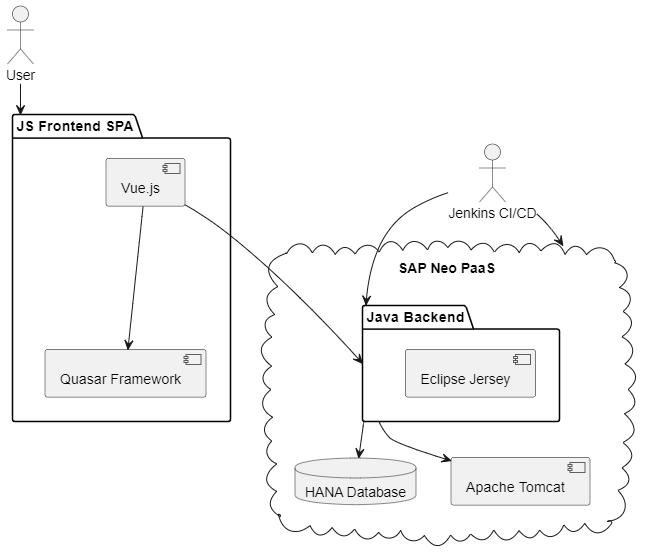
\includegraphics[width=.72\textwidth]{Bilder/architecture.png} 
	\caption{Die Abbildung zeigt die Architektur der Digital Heroes Lernplattform.}
	\label{fig:architecture}
\end{figure} 

Die Architektur der Web-App Digital Heroes mit den verschiedenen verwendeten Technologien
lässt sich in Frontend, Backend und DevOps unterteilen und 
ist in \autoref{fig:architecture} abgebildet. 
Es existieren zwei Instanzen der Architektur: ein Entwicklungs- und ein Produktivsystem. 

\subsubsection*{Frontend:}

Die Frontend-Anwendung der Digital Heroes Web-App ist als Single Page Application (SPA) konzipiert, 
die Vue.js und das Quasar Framework verwendet. 
Vue.js ist ein modernes JavaScript-Framework zum Erstellen von benutzerfreundlichen und reaktiven Webanwendungen.
Quasar ist ein weiteres Framework, das auf Vue.js aufbaut und zusätzliche Funktionen und Komponenten bereitstellt, 
um die Entwicklung von plattformübergreifenden Anwendungen zu erleichtern.
Vue.js nutzt die REST-API des Backends.

\subsubsection*{Backend:}

Das Backend der Web-App besteht aus einer Java-Anwendung, die Eclipse Jersey und Apache Tomcat verwendet. 
Eclipse Jersey ist eine Implementierung der JAX-RS-Spezifikation 
und ermöglicht die einfache Entwicklung von RESTful Web Services für Servlet Container. 
Apache Tomcat ist ein Servlet-Container, der als Webserver zum Bereitstellen von Java-Anwendungen dient
und das Java-Backend hostet.
Als Datenbank kommt die HANA-Datenbank zum Einsatz, die eine high-performance, in-memory relationale Datenbank ist 
und von SAP entwickelt wird. 
Das Java-Backend nutzt das Eclipse-Framework und die HANA-Datenbank um eine REST-API für das 
Vue.js-Frontend bereitzustellen. 

\subsubsection*{DevOps:}

Im Bereich der DevOps-Infrastruktur kommt Jenkins zum Einsatz, 
eine Open-Source-Automatisierungssoftware, 
die zur Implementierung von Continuous Integration und Continuous Deployment (CI/CD) verwendet wird. 
Jenkins ermöglicht die Automatisierung von Build- und Testprozessen sowie die Bereitstellung 
der Anwendung in einer kontrollierten und konsistenten Weise. 
Die Web-App wird auf der SAP Neo Platform-as-a-Service (PaaS) Cloud-Plattform gehostet, 
die eine skalierbare und einfach zu verwaltende Umgebung für die Bereitstellung 
und den Betrieb der Anwendung bietet.
Wird auf den Main-Branch des verwendeten Github-Respositories gepusht, bzw. eine Pull-Request gemerged,
startet Jenkins den CI/CD-Prozess und testet und deployed das neue Backend/Frontend auf der Entwicklungsinstanz. 
Änderungen im Frontend werden zudem direkt auf dem Produktivsystem deployed. 
Für Änderungen des Backends im Produktivsystem kann in SAP Neo ein neuer Release erzeugt werden, 
bei dem das Java-Backend der Entwicklungsinstanz auf das Produktivsystem kopiert wird. 


\section{Ist-Situation und warum die problematisch ist}

Das Entwickler-Team ist auf Deutschland und Australien aufgeteilt, 
was zu Kommunikationsschwierigkeiten und unterschiedlichen Arbeitszeiten führt. 
Dies erschwert die Zusammenarbeit und kann die Qualität der Software und die Effizienz 
der Entwicklungsprozesse beeinträchtigen.

Es gibt keine fest vorgegebenen Release-Zyklen; Releases finden nur statt, 
wenn ein neues Feature fertig ist. Dies kann zu unvorhersehbaren und unregelmäßigen Updates führen,
wodurch die Planung und das Management des Projekts schwieriger werden.
Außerdem werden Features möglicherweise nicht ausreichend vor einem Release getestet.

Releases werden oft freitags durch das australische Team durchgeführt. 
Dies ist problematisch, weil das Team in Australien möglicherweise nicht verfügbar ist, 
um eventuell auftretende Probleme sofort zu beheben, was zu längeren Ausfallzeiten führt. 
Das deutsche Team muss dann freitags die Probleme beheben oder einen Roll-Back veranlassen, 
wenn die Probleme zu groß sind. Insbesondere muss sich das deutsche Team aber erst 
in den Code des australischen Teams einlesen, was das Beheben der Fehler viel ineffizienter 
gestaltet, als wie wenn das australische Team diese Fehler beheben würde.

Es gibt keinerlei automatisierte Tests. Das bedeutet, 
dass die Qualität der Software nicht kontinuierlich überprüft wird, 
wodurch Fehler erst spät oder gar nicht entdeckt werden. Dies erhöht das Risiko drastisch, 
dass Fehler in die Produktion gelangen, was zu einer schlechteren Benutzererfahrung führt.

Viele Bugs gelangen in die Produktionsumgebung, 
was häufig auf die fehlenden Tests zurückzuführen ist, 
wodurch oft Hot-Fixes notwendig sind. Dies zeigt, 
dass der Entwicklungsprozess und die Qualitätssicherung unzureichend sind 
und die Softwarequalität leidet. Außerdem sind die Hot-Fixes selbst ungetestet 
und sehr überhastet erstellt worden, was wiederum zu mehr Bugs führen kann. 
Auch betreffen diese Bugs gelegentlich völlig andere Teile des Systems und fallen nicht sofort auf.
Zu allem Überfluss werden diese Hot-Fixes mit diesen gefährlichen Bugs direkt auf das Produktiv-System 
deployed. 

Der CI/CD-Prozess für das Deployment auf der Entwicklungsinstanz dauert 15 Minuten. 
Das ist eine lange Wartezeit, die den Entwicklungsprozess verlangsamt und zu einer geringeren Produktivität führt.
Zur Verschlimmerung der Lage kann das Backend nicht auf dem lokalen Rechner gestartet werden, 
da die HANA-Datenbank nicht lokal gehostet werden kann und kein Mock existiert. 
Dies erschwert die lokale Entwicklung und das Testen, 
was die Effizienz der Entwickler stark beeinträchtigt und die Qualität der Software gefährdet, 
da Neuerungen weniger getesetet werden, weil der Testprozess so frustrierend für die Entwickler ist.

Die Codequalität ist in einem schrecklichen Zustand: Viele duplikative Code-Stücke, 
wenig Struktur und keine Aufteilung der Architektur in Schichten. 
Es wird immer gegen Implementierungen programmiert, anstatt gegen Abstraktionen. 
Dies führt zu einer schlechteren Wartbarkeit, schlechterer Lesbarkeit, 
erschwert das Testen, da Mocks und Fakes nicht möglich sind,  
erhöht die Fehleranfälligkeit und erschwert die Einarbeitung neuer Teammitglieder, 
was insbesondere in dem Projekt ein Problem ist, da oft Studenten hier arbeiten, 
die nicht für lange Zeit eingebunden sind und dadurch hohe Fluktation besteht. \\
Desweiteren ist der Code ist oft fehleranfällig und unleserlich, 
zum Beispiel durch 40-50 Zeilen lange, 
verschachtelte SQL-Statements, die viel Code-Duplikate enthalten. 
Dies führt zu einer schlechteren Wartbarkeit und macht es schwieriger, 
Fehler zu erkennen und zu beheben, da oft nicht alle Duplikate angepasst werden.

Es gibt keine Code-Reviews, was bedeutet, dass keine systematische Überprüfung der Codequalität 
stattfindet. Dies erhöht die Wahrscheinlichkeit von Fehlern und mindert damit die Qualität der Software.

Obwohl ein Kanban-Board mit Tasks und Prioritäten verwendet wird, 
gibt es kein Sprint-Planning und kein Sprint-Review. 
Dies führt zu einer schlechteren Planung und Kontrolle der Arbeit 
und beeinträchtigt die Effizienz des Entwicklungsprozesses, weil keine klarere Absteckung der 
Aufgaben stattfindet und nicht bewertet wird, wie der vorangegangene Sprint lief.

Die Scrum-Meetings finden zweimal pro Woche statt, 
aber mit der ganzen Abteilung (nicht nur Entwickler, sondern auch Designer, Manager, Content-Moderatoren usw.). 
Dadurch werden diese Meetings sehr ineffizient, 
da nicht alle Teilnehmer direkt am Entwicklungsprozess beteiligt sind. 
Dies führt zu einer schlechteren Kommunikation und Koordination innerhalb des Entwicklerteams 
und verlangsamt den Entwicklungsprozess enorm, da die Mitglieder in dem Meeting gebunden sind, 
obwohl ein Großteil der Inhalte nicht relevant für das jeweilige Mitglied sind. 
Dadurch wird viel Zeit verschwendet.

Insgesamt sind die identifizierten Probleme im Bereich des Software-Qualitäts-Managements
und Entwicklungsprozesse ein erhebliches Hindernis für die Erreichung einer 
hohen Softwarequalität und einer effizienten Arbeitsweise. Um die Situation zu verbessern, 
müssen die genannten Probleme adressiert und Lösungen gefunden werden, 
die zu einer besseren Organisation, Kommunikation und Qualitätssicherung führen.

\section{Mögliche Ursachen für die identifizierten Probleme}

Die geschilderten Probleme in Bezug auf das Software-Qualitäts-Management 
und den Entwicklungsprozess sind vielfältig und komplex. Es gibt mehrere mögliche Gründe, 
die zu diesen Schwierigkeiten geführt haben. Um diese Probleme nachhaltig zu lösen, 
müssen die Gründe verstanden werden, die dazu geführt haben, ansonsten werden nur 
Symptome behandelt und die Probleme nicht an der Wurzel angegangen. 
Eine kritische Untersuchung der Situation zeigt folgende mögliche Ursachen:

Unerfahrene Projektleitung: Eine der Hauptursachen für die identifizierten Probleme 
ist eine unerfahrene oder teilweise auch überforderte Projektleitung. 
Da die festangestellte Projektleitung wenig Erfahrung im Bereich Softwareentwicklung 
und Projektmanagement hat, führt dies dazu, dass sie die bestehenden Probleme nicht versteht 
oder realisiert. Dies führt zu einer unzureichenden Organisation, 
fehlender Prozesskontrolle und wenig Vertsändnis für Ressourcenaufwand, welcher für Qualitätssicherung 
eingesetzt wird.

Hoher Anteil unerfahrener Studenten: Die schlechte Qualität der Software 
und der Entwicklungsprozesse könnte auch auf den hohen Anteil unerfahrener Studenten zurückzuführen sein, 
die in der Abteilung arbeiten. Da diese Studenten nur für eine begrenzte Zeit
im Projekt tätig sind und nicht die erforderliche Erfahrung haben, 
kann dies zu einer hohen Mitarbeiterfluktuation und einer unzureichenden Kontinuität in der Entwicklung führen. 
Dies wirkt sich negativ auf die Qualität der Software und die Effizienz der Entwicklungsprozesse aus.

Fehlende Verantwortung und Initiative: Ein weiterer Grund für die identifizierten Probleme könnte sein, 
dass sich keines der Teammitglieder verantwortlich fühlt, die Probleme zu adressieren und zu verbessern. 
Dies kann auf mangelnde Kommunikation (insbesondere zwischen deutschem und australischem Team), 
fehlende Anreize oder eine unklare Rollenverteilung 
innerhalb des Teams zurückzuführen sein. Wenn niemand das Gefühl hat, 
für die Qualität der Software und die Effizienz der Entwicklungsprozesse verantwortlich zu sein, 
wird es schwierig sein, die Situation nachhaltig zu verbessern.

Kommunikationsschwierigkeiten: Die Aufteilung des Entwicklerteams auf verschiedene Standorte, 
wie Deutschland und Australien, kann zu Kommunikationsschwierigkeiten führen. 
Zeitverschiebung, kulturelle Unterschiede und eine eingeschränkte Möglichkeit 
für persönliche Treffen führen dazu, dass Missverständnisse entstehen und Entscheidungen 
nicht effektiv getroffen werden.

Hoher Druck durch Nutzeranforderungen: Die Nutzer fordern häufig schnell neue Features, 
was den Druck auf die Studenten erhöht, diese Anforderungen umzusetzen. 
Da die Studenten möglicherweise nicht in der Lage sind, 
"nein" zu sagen oder Prioritäten angemessen zu setzen, 
kann dies zu einer Vernachlässigung von wichtigen Aspekten wie Qualitätssicherung, 
Testentwicklung und Code-Reviews führen. 

Fokus auf Feature-Entwicklung statt Testentwicklung: Die studentischen Entwickler legen den Fokus eher auf 
die Implementierung neuer Features, anstatt auf das Schreiben von Tests, 
da das Erstellen neuer Funktionen als "spannender" oder "produktiver" wahrgenommen wird. 
Außerdem wird durch die fehlende Erfahrung das Schreiben von Tests und anderen 
Qualitätssicherungsmaßnahmen als eher unwichtig eingeschätzt. 

Mangel an Vollzeitentwicklern: Da es keine Vollzeitentwickler oder Senior Development-Experten gibt,
wird die Entwicklungsleitung nicht durch einen erfahrenen Entwickler übernommen, 
der die nötige Führung für die jungen studentischen Junior Entwickler bieten könnte.


% ---- Literaturverzeichnis
\cleardoublepage
\renewcommand*{\chapterpagestyle}{plain}
\pagestyle{plain}
\pagenumbering{Roman}                   % Römische Seitenzahlen
\setcounter{page}{\numexpr\value{savepage}+1}
\printbibliography[title=Literaturverzeichnis]

% ---- Anhang
\appendix
%\chapter{Anhang}

\section{Architekturen}

\pagebreak

\section{Quelltext-Implementation}
%\clearpage
%\pagenumbering{Roman}  % römische Seitenzahlen für Anhang

\newpage
\end{document}
